\section{Heavy edges}
\label{section:heavy_edges}

\subsection*{Purpose}

\paragraph{}
To study the inter-accuracy of top-k heavy edges between the original stream and the graph sketches.

\paragraph{}
Inter-accuracy for top-k elements has been defined in \autoref{section:metrics_inter}.

\subsection*{Results}

\begin{figure}[H]
    \centering 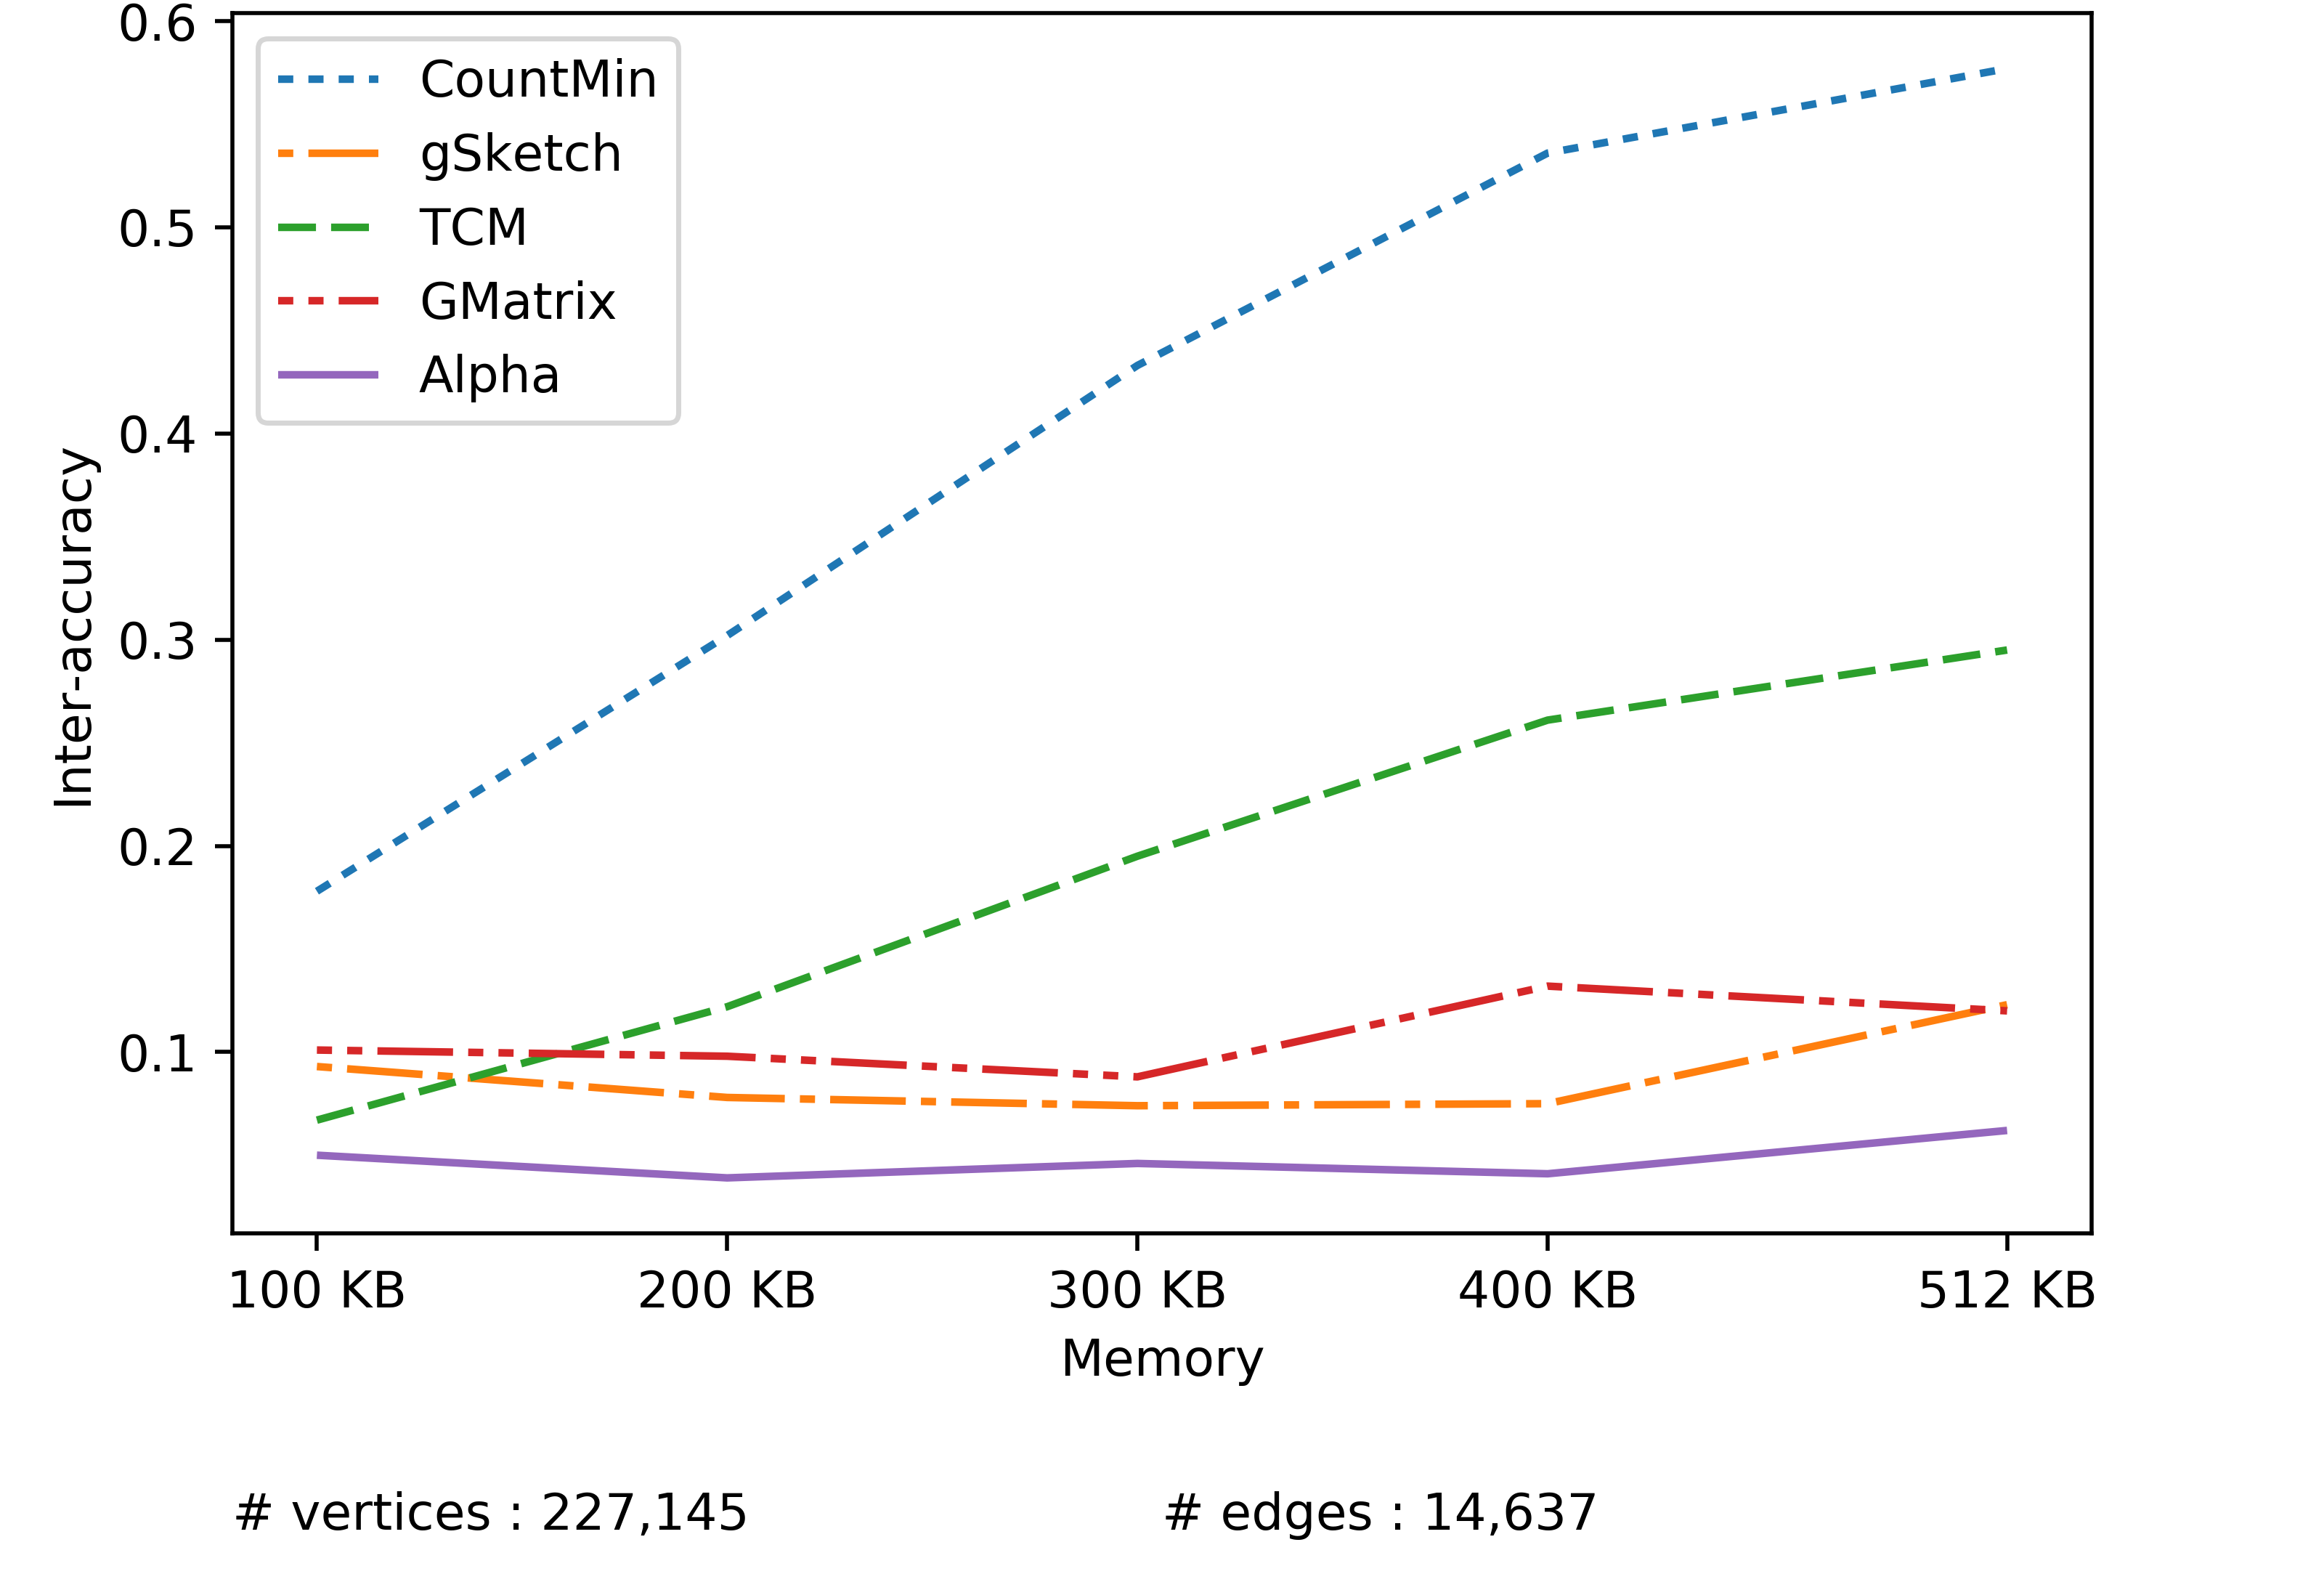
\includegraphics[width=0.85\textwidth]{results/he/unicorn-wget-he}
    \vspace{-0.5cm}
    \caption{Inter accuracy of heavy edges vs Memory for unicorn-wget dataset}
    \label{fig:unicorn-wget-he}
\end{figure}

\begin{figure}[H]
    \centering 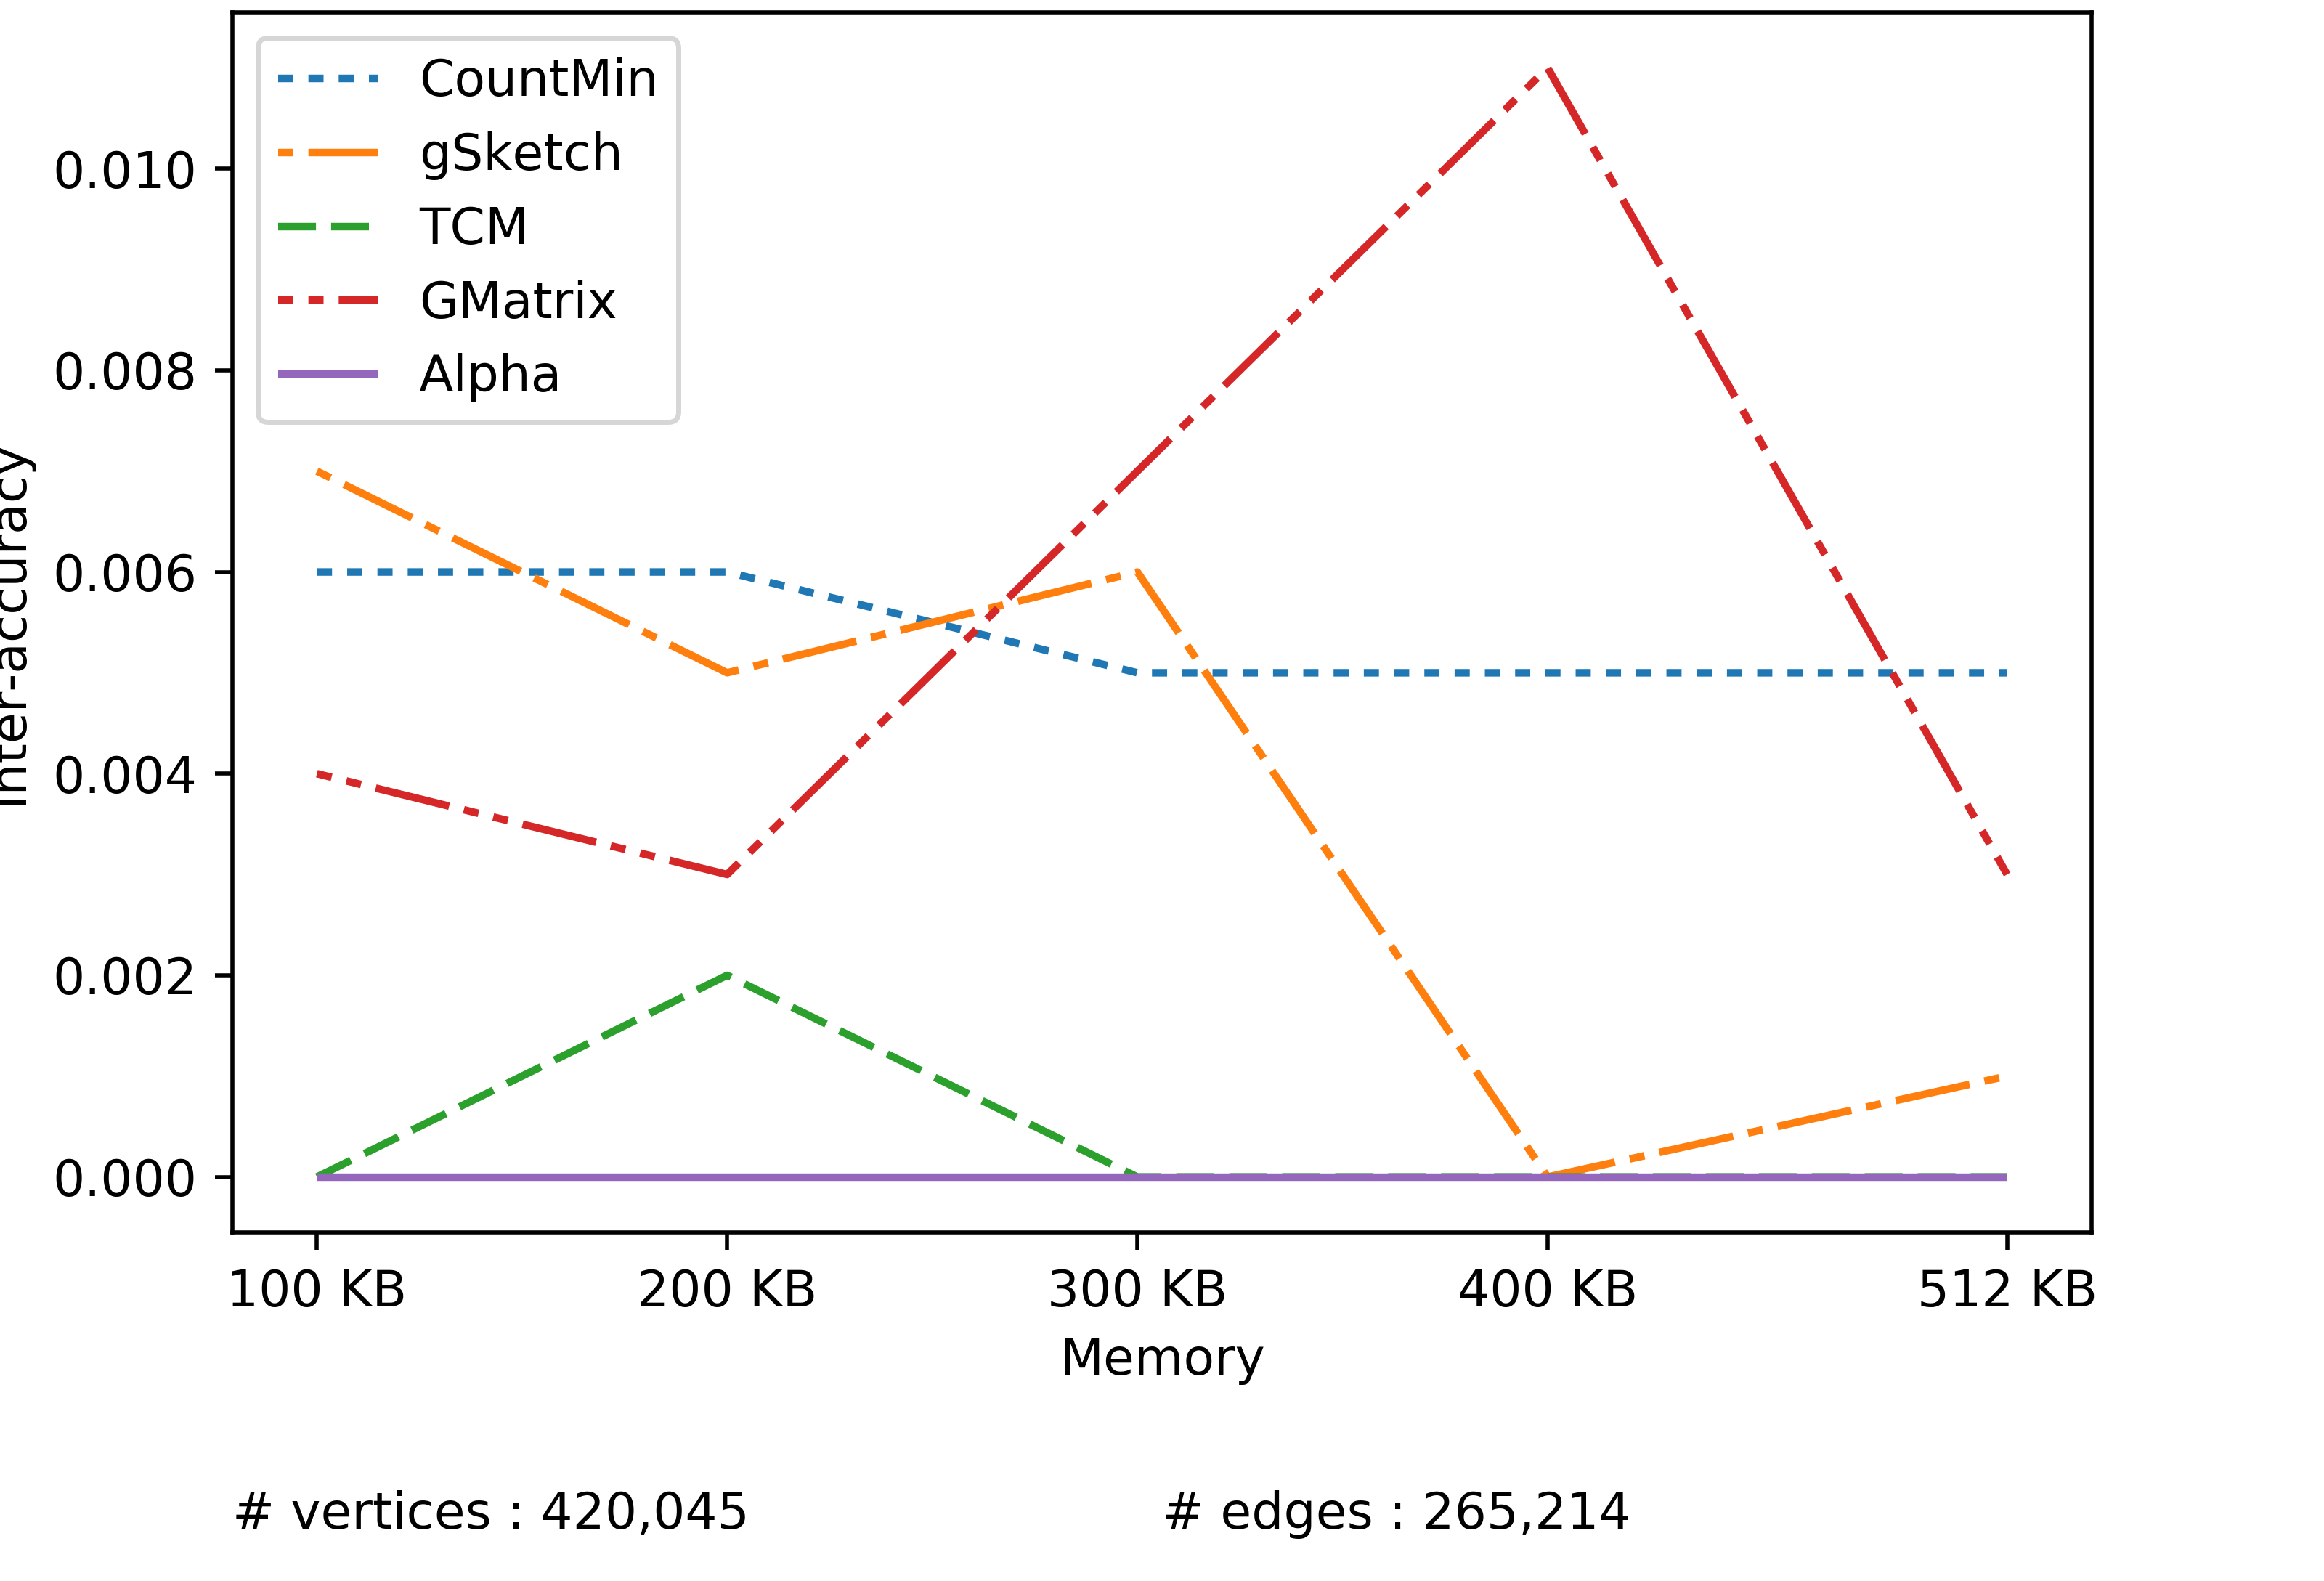
\includegraphics[width=0.85\textwidth]{results/he/email-EuAll-he}
    \vspace{-0.5cm}
    \caption{Inter accuracy of heavy edges vs Memory for email-EuAll dataset}
    \label{fig:email-EuAll-he}
\end{figure}

\begin{figure}[H]
    \centering 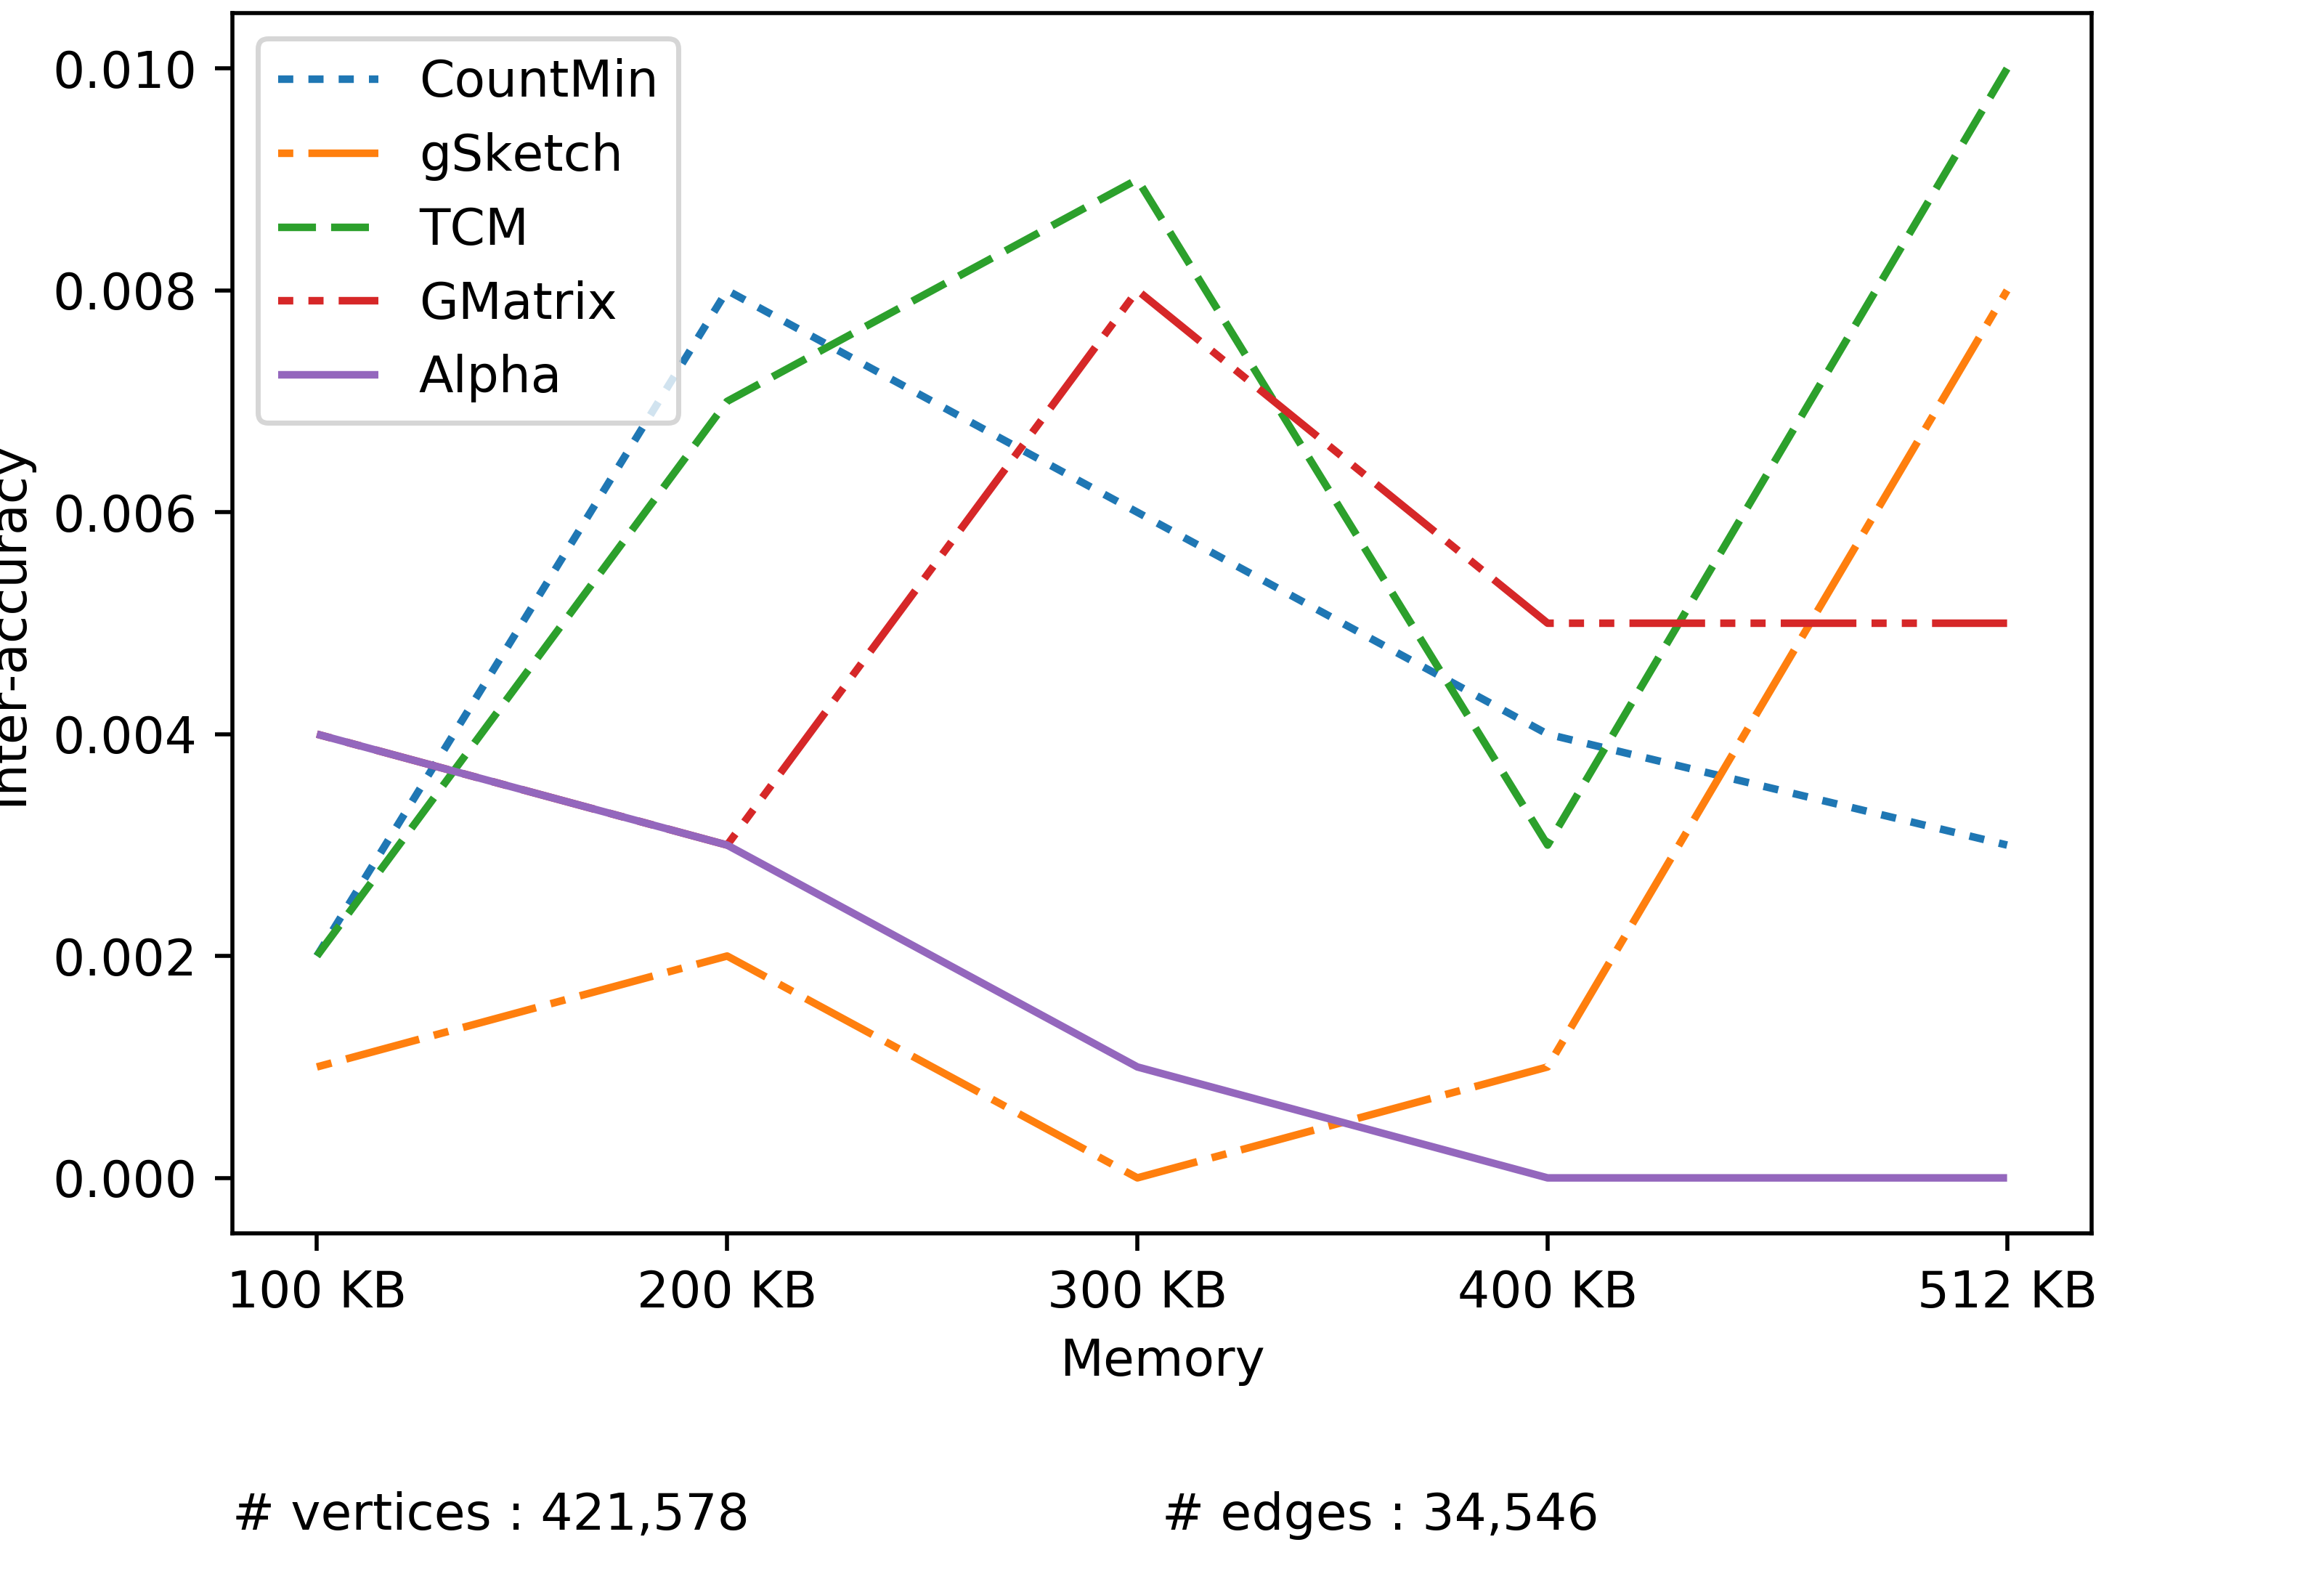
\includegraphics[width=0.85\textwidth]{results/he/cit-HepPh-he}
    \vspace{-0.5cm}
    \caption{Inter accuracy of heavy edges vs Memory for cit-HepPh dataset}
    \label{fig:cit-HepPh-he}
\end{figure}

\begin{figure}[H]
    \centering 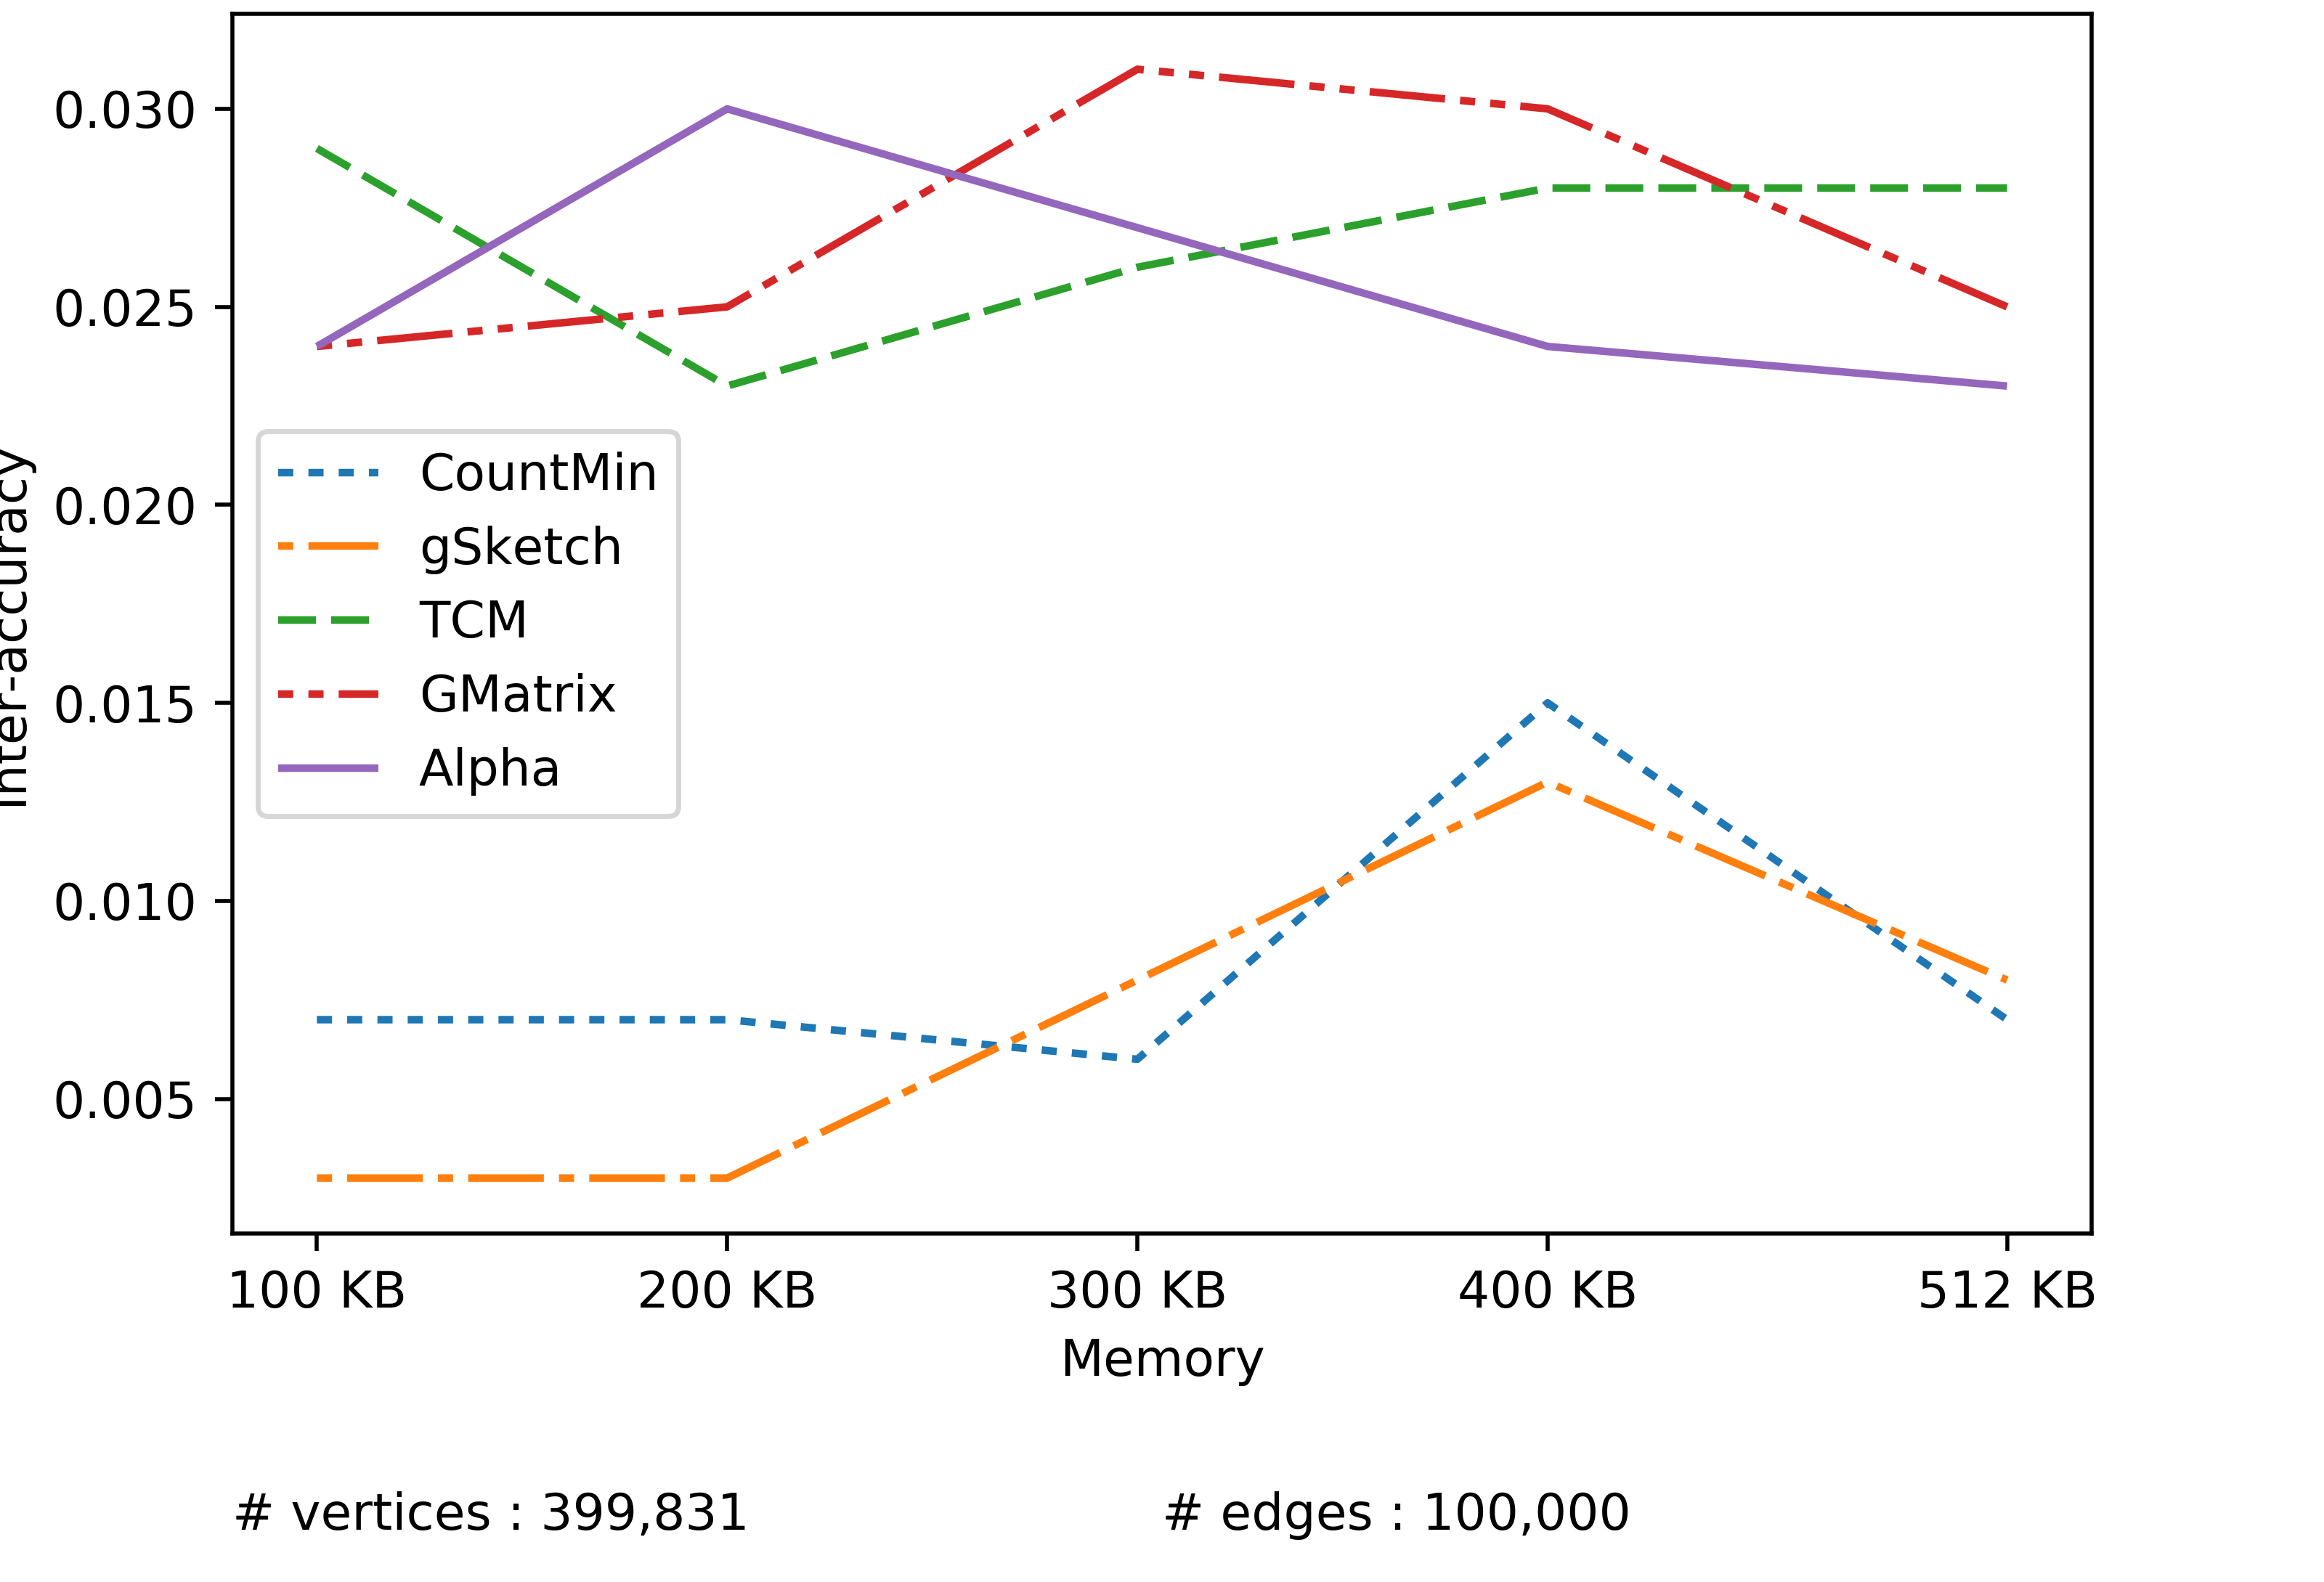
\includegraphics[width=0.85\textwidth]{results/he/gen-scale-free-he}
    \vspace{-0.5cm}
    \caption{Inter accuracy of heavy edges vs Memory for gen-scale-free dataset}
    \label{fig:gen-scale-free-he}
\end{figure}

\begin{figure}[H]
    \centering 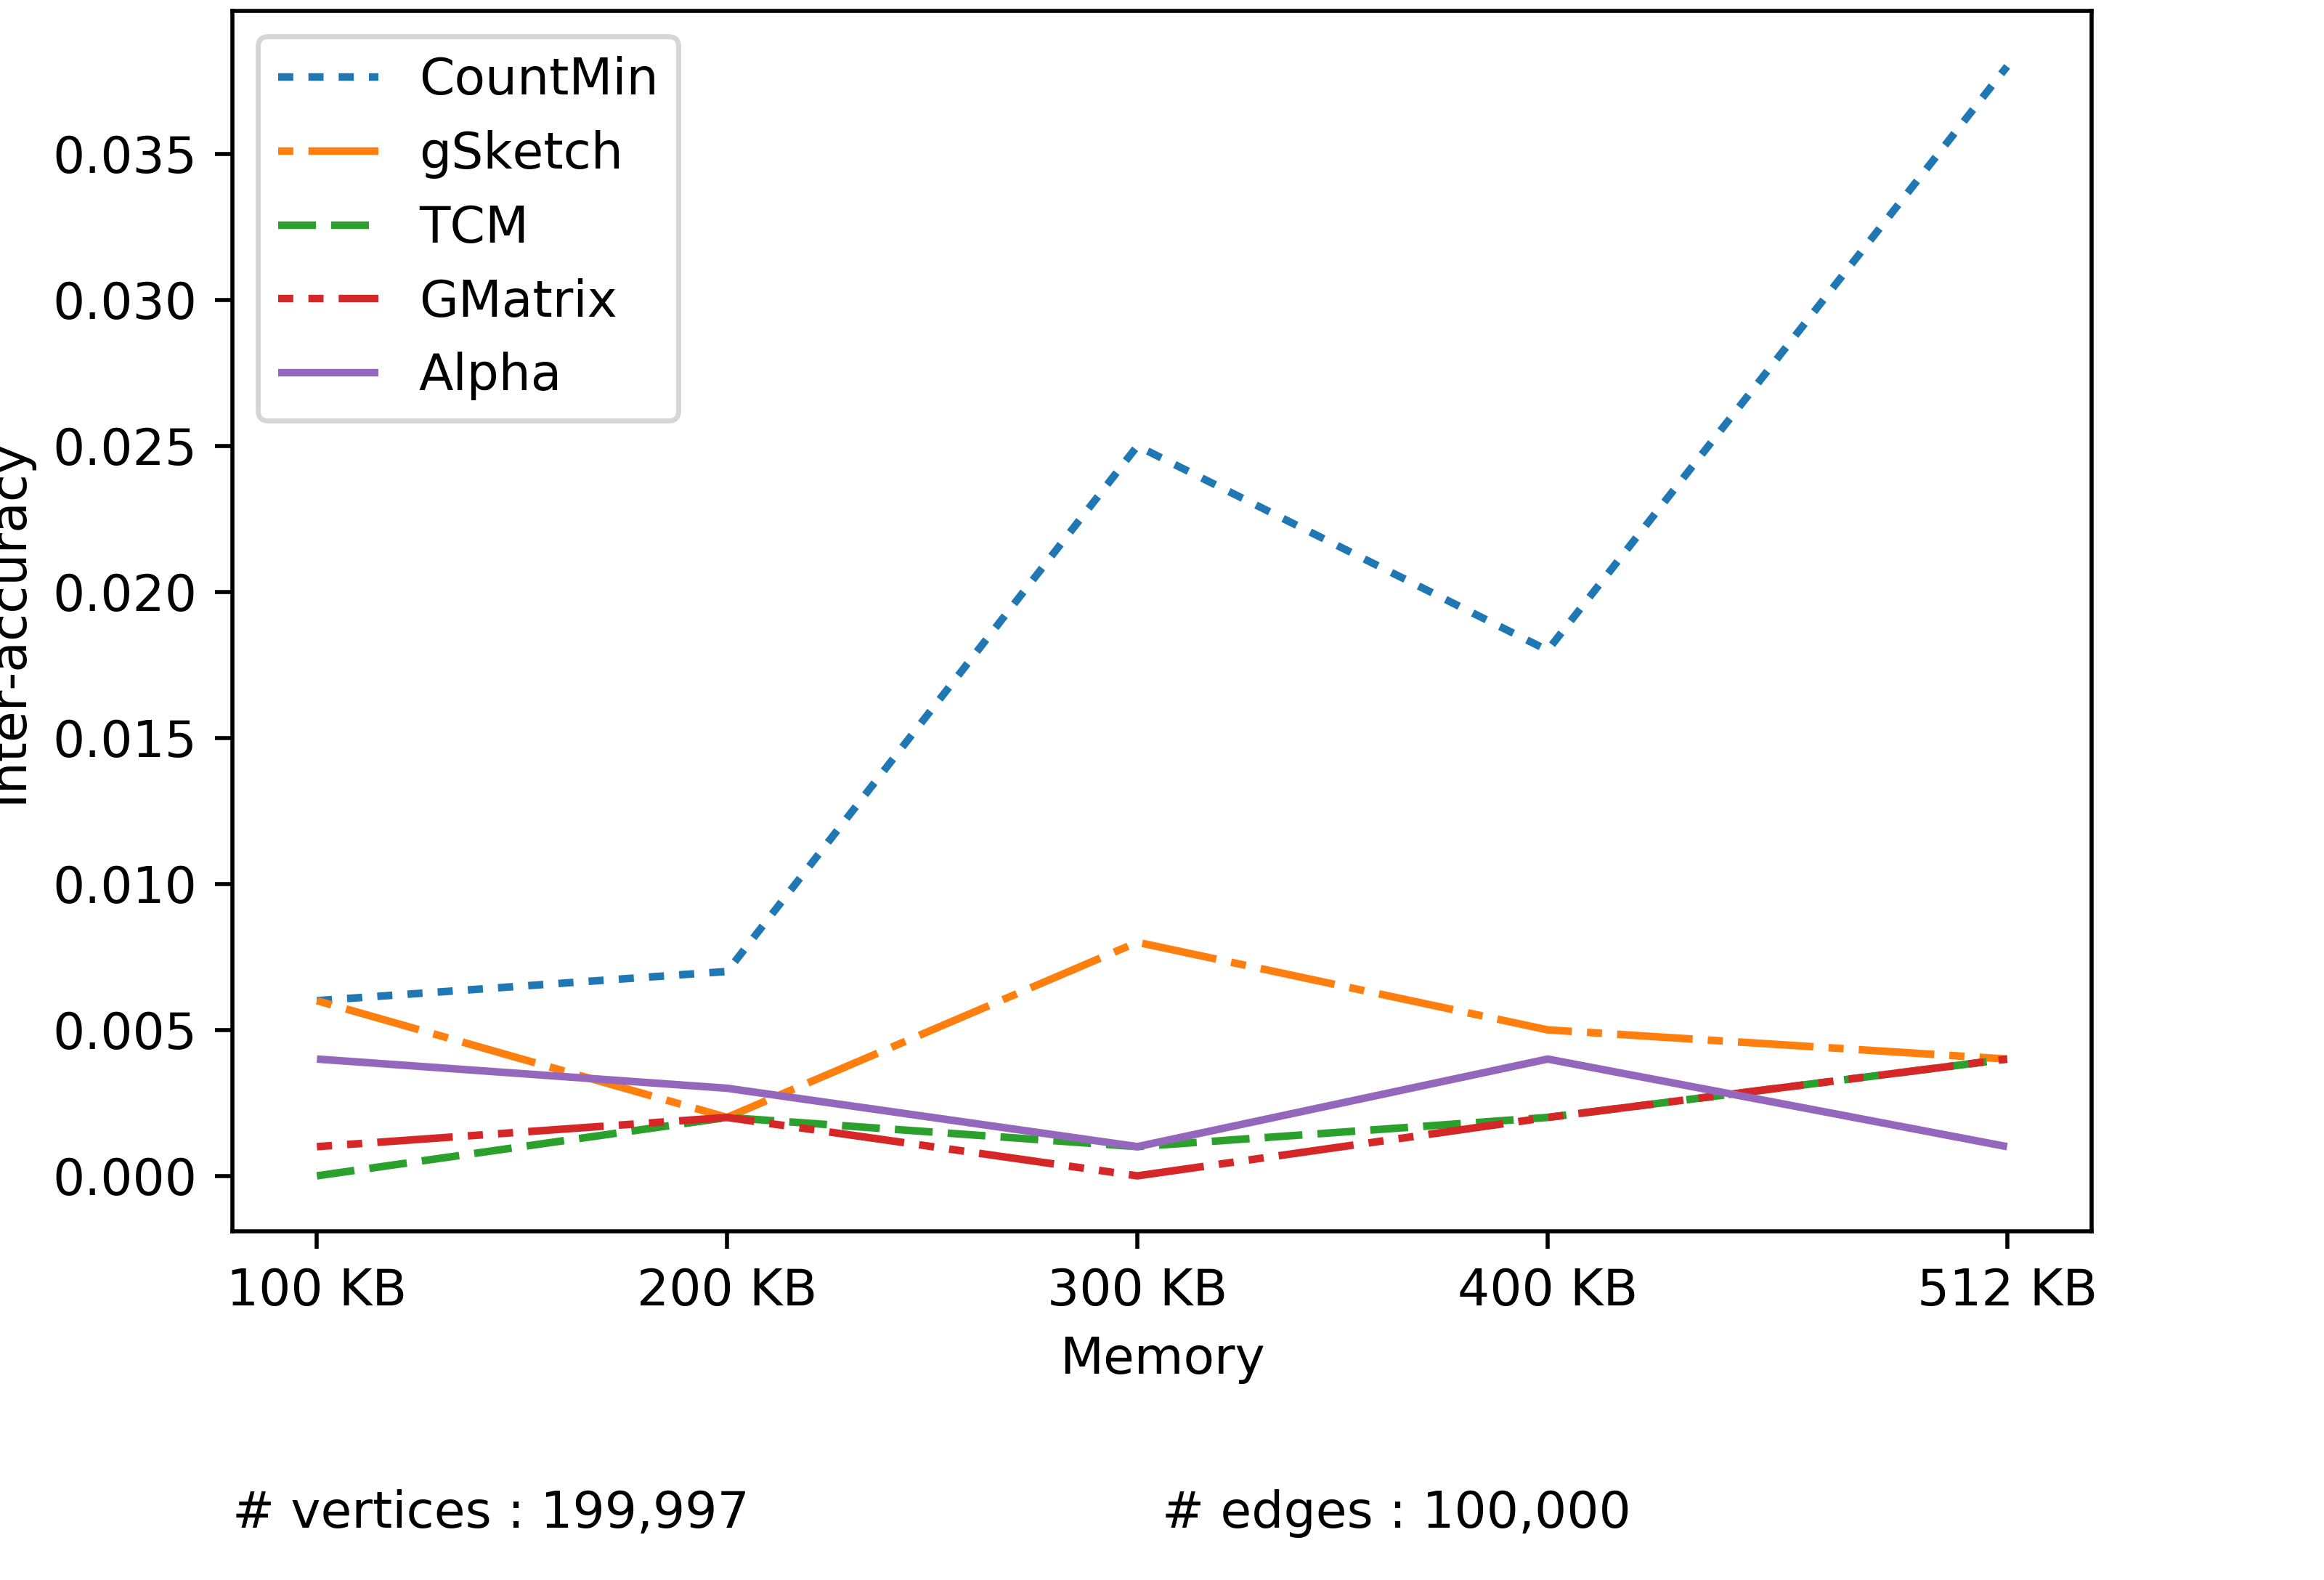
\includegraphics[width=0.85\textwidth]{results/he/gen-small-world-he}
    \vspace{-0.5cm}
    \caption{Inter accuracy of heavy edges vs Memory for gen-small-world dataset}
    \label{fig:gen-small-world-he}
\end{figure}

\subsection*{Observations and inferences}

\paragraph{}
Both the partitioned sketches, gSketch and Alpha has shown comparably low inter accuracies for top-k heavy edge queries for the datasets, unicorn-wget in \autoref{fig:unicorn-wget-he}, email-EuAll in \autoref{fig:email-EuAll-he} and cit-HepPh in \autoref{fig:cit-HepPh-he}. Thus we can infer that the partitioning of the sketches has negatively affected the performance of heavy edge queries.

\paragraph{}
The accuracy of Alpha is relatively better in the generated gen-scale-free and gen-small-world datasets for some sketch sizes, which strictly follow the power law distribution properties.

\paragraph{}
The accuracy of the CountMin sketch with respect to heavy edge queries have suffered in comparison to the results of the heavy node queries in the \autoref{section:heavy_nodes}. However CountMin sketch can still be proposed as a reliable sketch in answering heavy edge queries for graph streams in general.